\documentclass[12pt]{article}
\usepackage{amsmath}
\usepackage{enumerate}
\usepackage[margin=1in]{geometry}
\usepackage{booktabs, multicol, multirow}
\usepackage[capposition=top]{floatrow}
\usepackage{graphicx}
\usepackage{csquotes}
\usepackage{lscape}
\usepackage{array}
\usepackage{caption}
\usepackage{subcaption}
\usepackage{dcolumn}
\usepackage{varwidth}
\usepackage{endnotes}
\usepackage{indentfirst}
\usepackage[hyphens]{url}
%\usepackage{breakurl} 
\usepackage[breaklinks]{hyperref}
\usepackage[table]{xcolor}
\usepackage{setspace}
\usepackage{alltt}
\pagestyle{empty}



\begin{document}


\begin{figure}[h!]
\caption*{\bf Figure 1. Section scores, by Prior Achievement and Future Commitment.}
\centering
    \begin{subfigure}[b]{0.4\textwidth}
        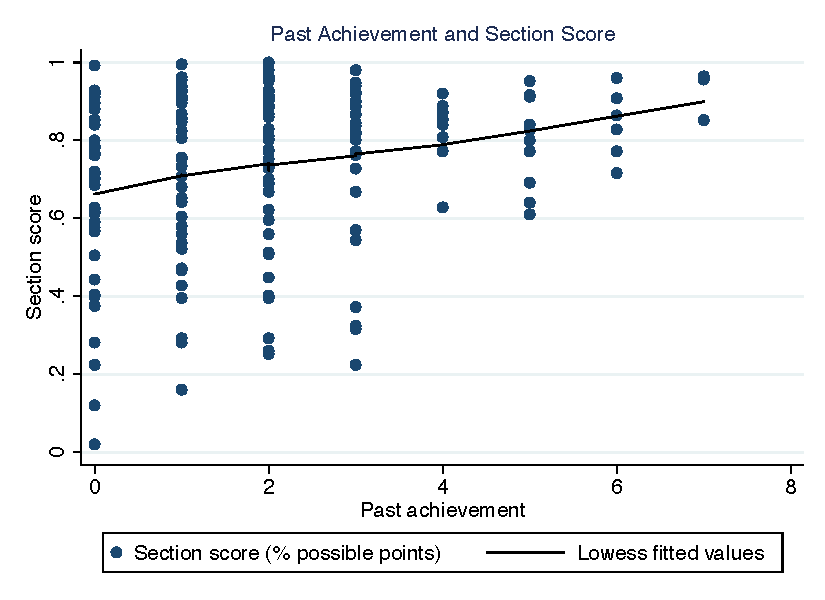
\includegraphics[width=\textwidth]{scatter7.pdf}
    \end{subfigure}
    \begin{subfigure}[b]{0.4\textwidth}
        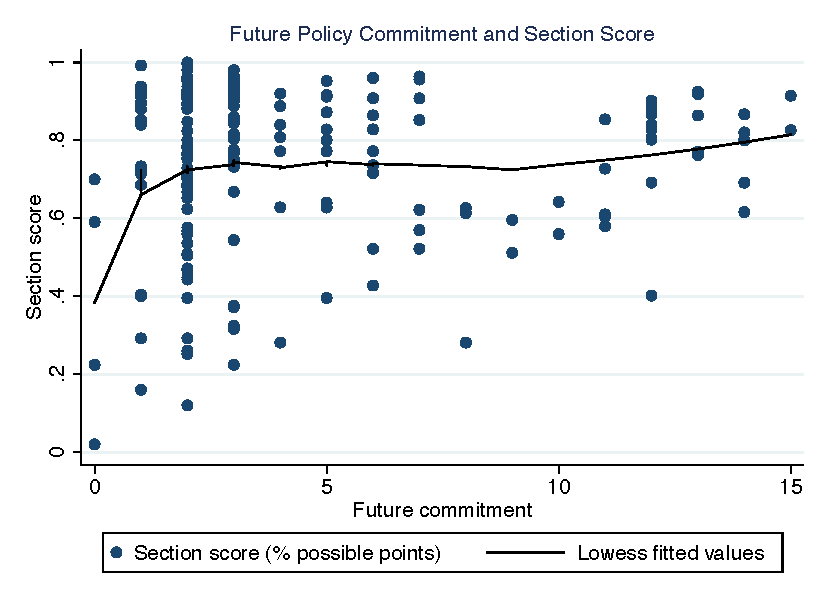
\includegraphics[width=\textwidth]{scatter8.pdf}
    \end{subfigure}
\begin{minipage}{\textwidth} 
\vspace{2mm}
\begin{singlespace}
{\footnotesize \textit{Notes:} Dots represent state-by-section observations from the latest phase of 1 or 2 in which a state applied for RttT, for all applicants (winners and losers). Included sections are A, C, D, E, and F. For both panels, the y-axis represents the section score that applications received as a proportion of possible points they could earn on that section. On the left panel, the x-axis identifies the number of past achievements of coded RttT policies within the relevant section. On the right panel, the x-axis identifies the number future commitments of coded RttT policies within the relevant section.}
\end{singlespace}
\end{minipage}
\end{figure}

\clearpage

\begin{figure}[h!]
\caption*{\bf Figure 2. Trends in RttT Policy Mentions.}
\begin{minipage}{.85\textwidth} 
\begin{center}
     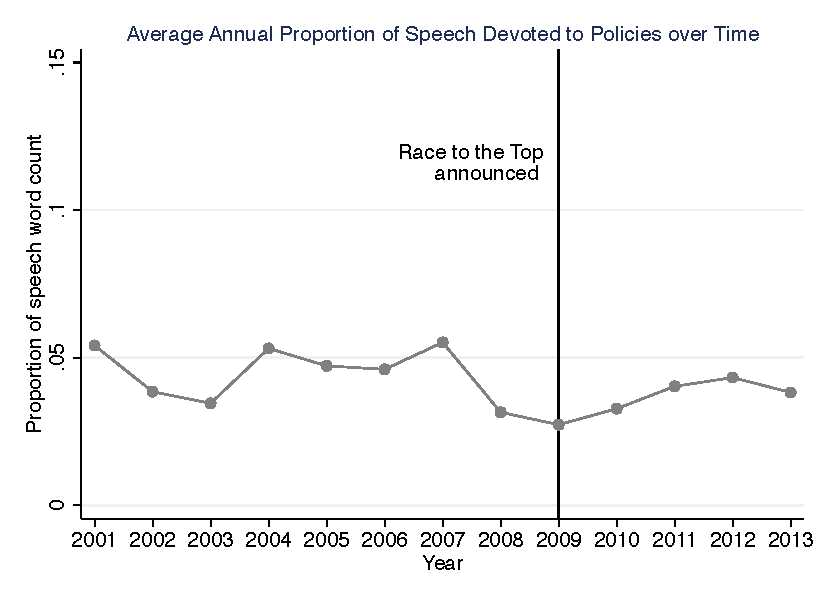
\includegraphics[width=.49\textwidth]{scatter_speeches_mean.pdf}
     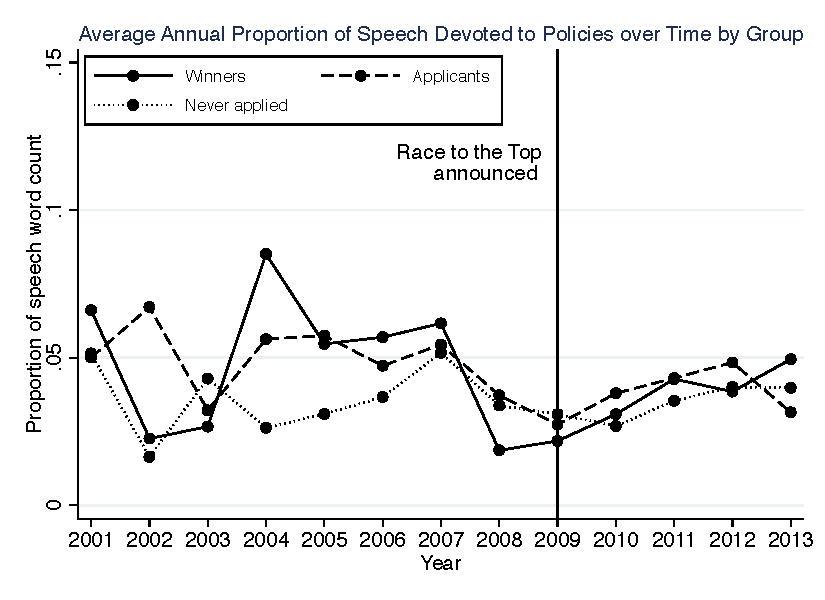
\includegraphics[width=.49\textwidth]{scatter_speeches_mean_all.pdf}
     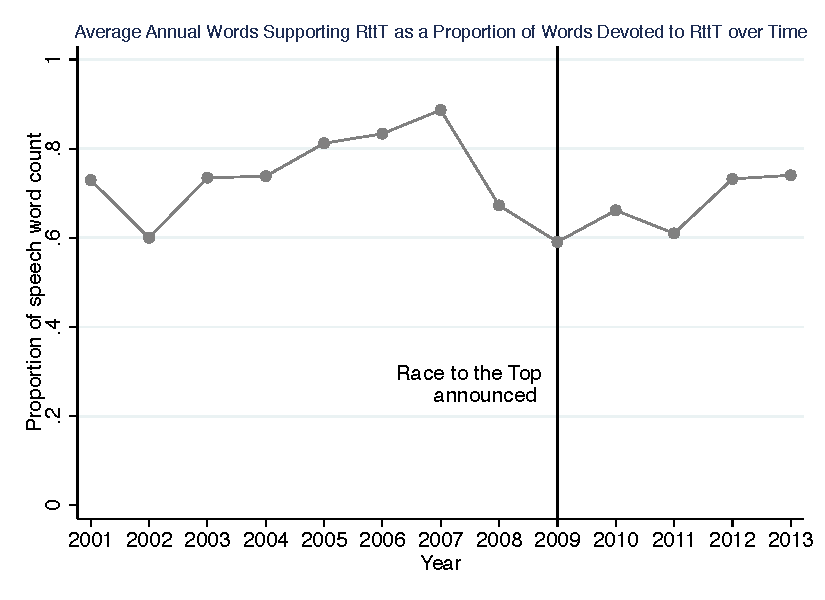
\includegraphics[width=.49\textwidth]{scatter_speeches_mean_pro.pdf}
     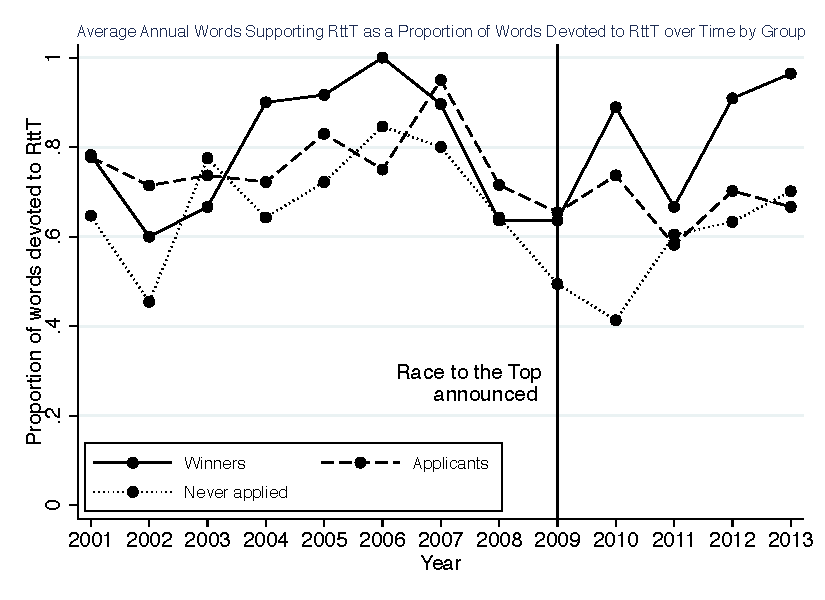
\includegraphics[width=.49\textwidth]{scatter_speeches_mean_all_pro.pdf} 
\end{center}
{\footnotesize \textit{Notes:} In the top panels, the unit of analysis is the total number of words devoted to all RttT priorities as a proportion of all words in the speech. In the bottom panels, the unit of analysis is the number of words in support of all RttT priorities as a proportion of the number of total words devoted to those priorities in the speech. Winners are states that won in any round of the competition and applicants are states that applied in at least one round but never won. Because this definition is not dynamic over time, Round 3 (2011) winners that had not yet won in 2010 are still counted as winners in that year.  \par}
\end{minipage}
\end{figure}

\clearpage

\begin{figure}[h!]
\caption*{\bf Figure 3. Trends in RttT Policy Enactment.}
\begin{minipage}{.85\textwidth} 
\begin{center} 
    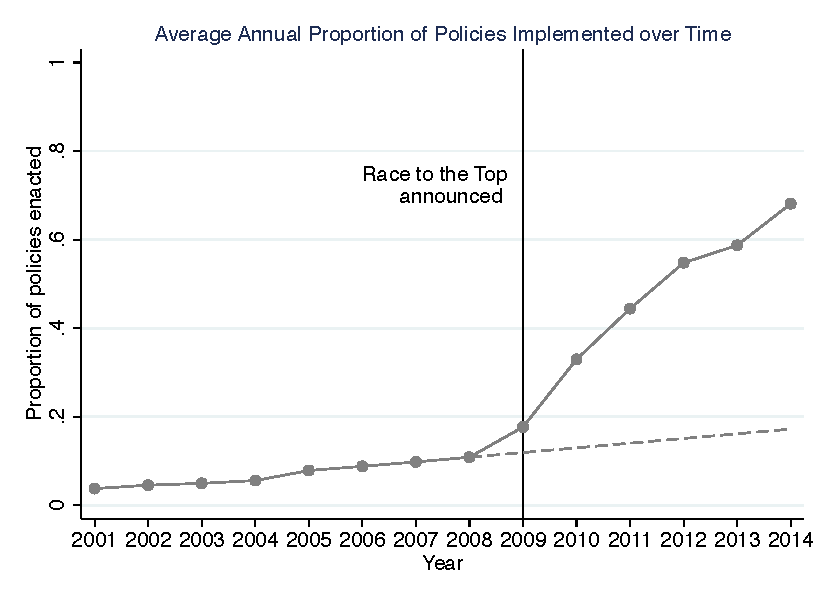
\includegraphics[width=.49\textwidth]{scatter_leghist_mean.pdf}
    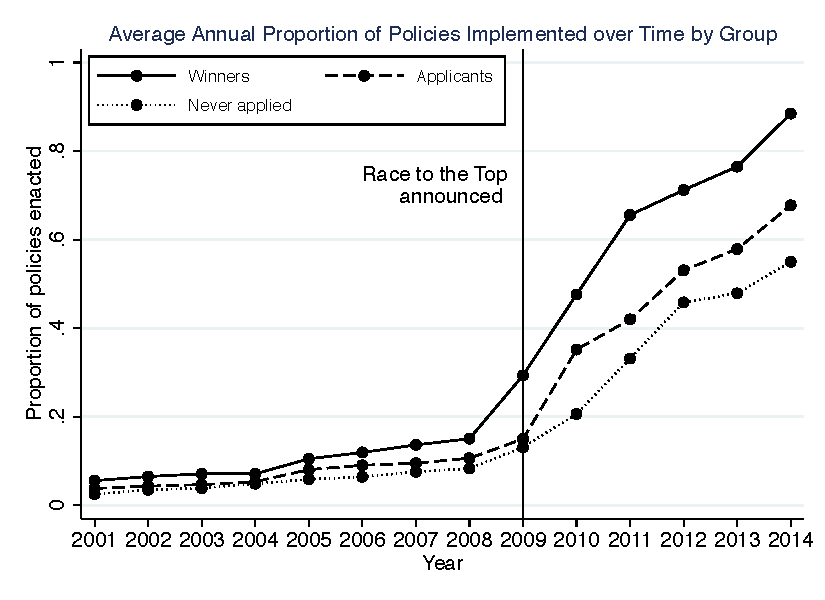
\includegraphics[width=.49\textwidth]{scatter_leghist_mean_all.pdf}
\end{center}
{\footnotesize \textit{Notes:} Unit of analysis is the proportion of RttT policies on the book in a given year. The dotted line in the left panel extends the trend line from 2007 to 2008. Winners are states that won in any round of the competition and applicants are states that applied in at least one round but never won. Because this definition is not dynamic over time, Round 3 (2011) winners that had not yet won in 2010 are still counted as winners in that year. The main policy areas covered by RttT were announced on March 7, 2009. All but one of the policies represented in the 2009 data point above were implemented before that date. The 2014 data point represents policy implementation as of April 2014. \par}
\end{minipage}
\end{figure}

\clearpage

\begin{landscape}
\begin{figure}[h!]
\footnotesize
\captionsetup{justification=centering}
\caption*{{\bf Figure 4. Q-Q Plots of Balance on Section Score \\ Exact Matching on Year and Policy Domain, Nearest Neighbor Matching on Section Score.}}\label{fig:qq_type}
\begin{minipage}{\textwidth} 
\begin{center}
    \begin{subfigure}[label]{\textwidth}
    \caption*{Comparison 1: 2010-11, treated observations are Phase 1 and 2 winners and untreated observations are all others}
    \centering
         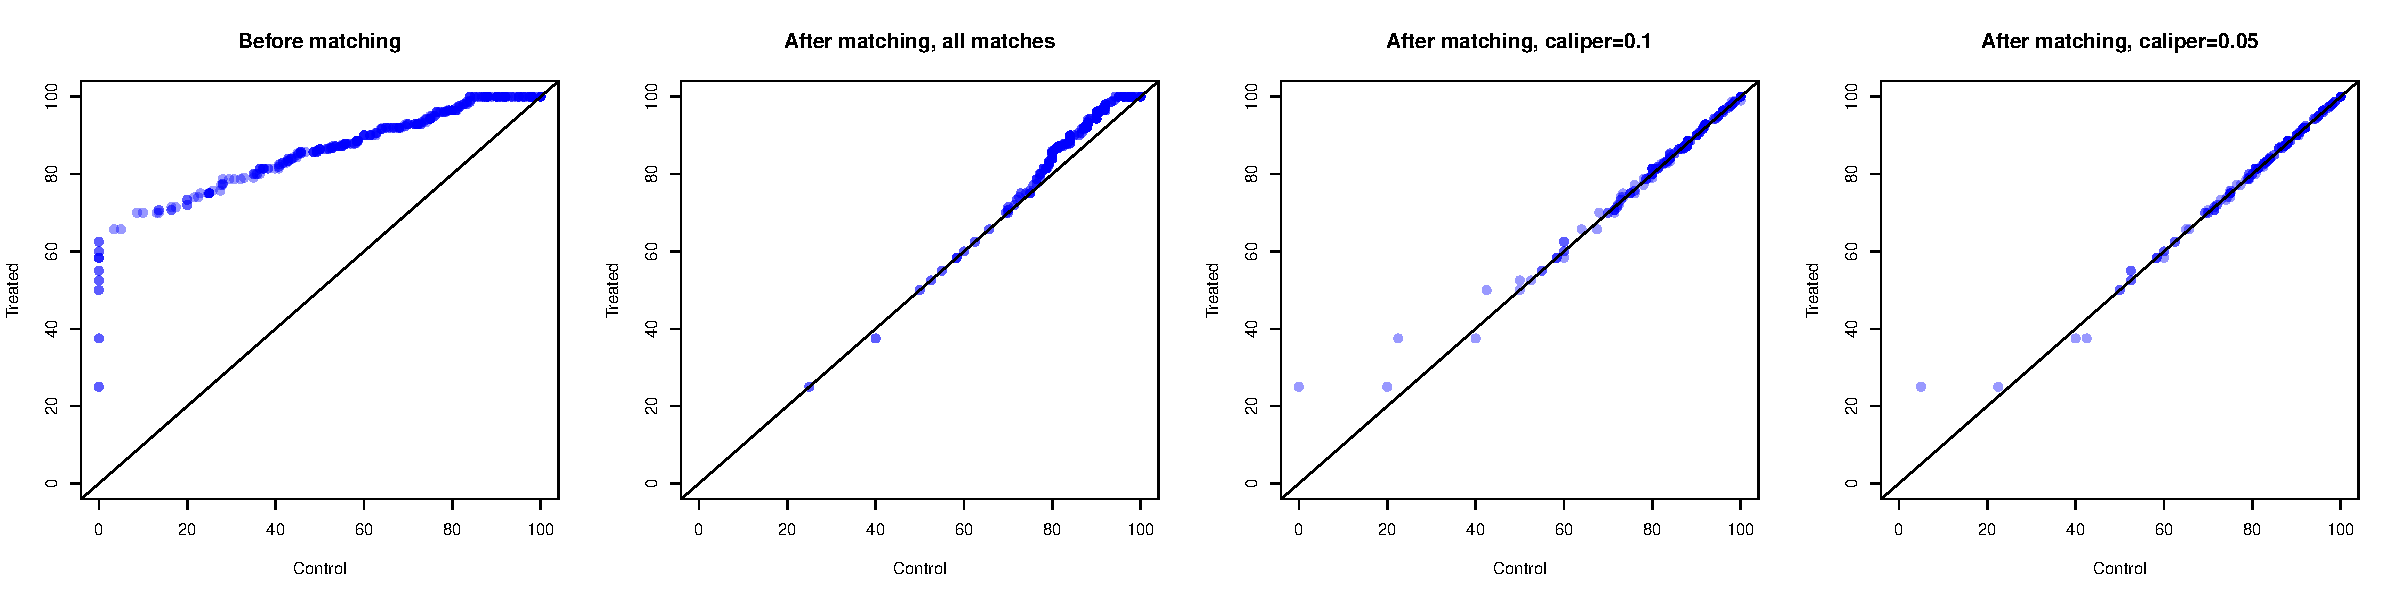
\includegraphics[width=.7\textwidth]{plots_type_1.pdf}
    \end{subfigure}
     \begin{subfigure}[label]{\textwidth}
     \caption*{Comparison 2: 2012-13, treated observations are Phase 3 winners and untreated observations are applicants that never won}
     \centering
     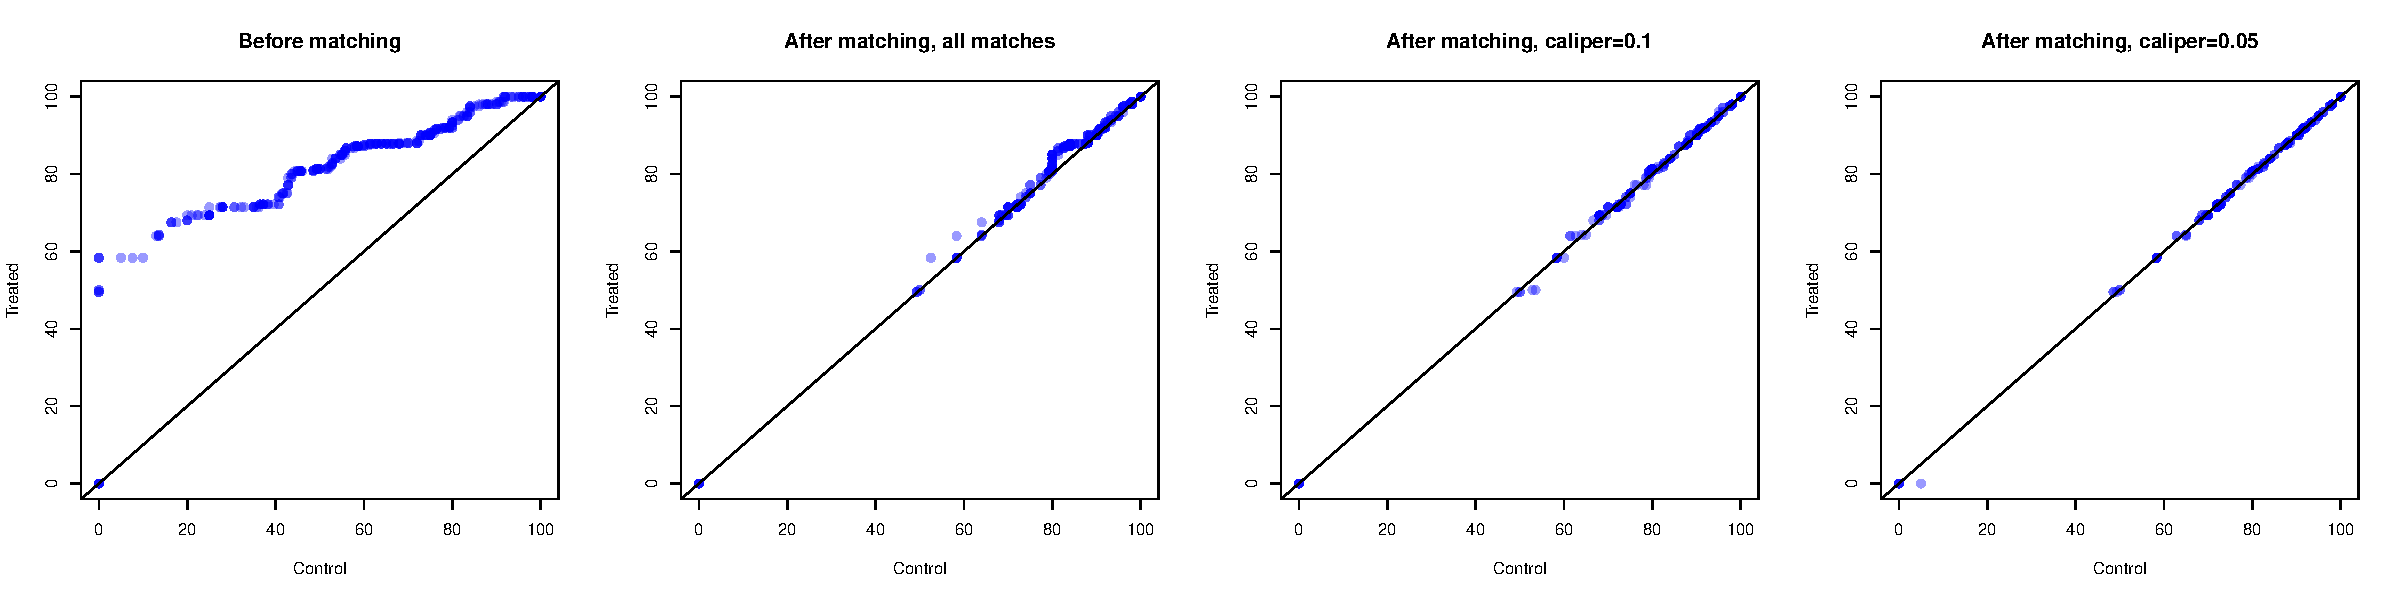
\includegraphics[width=.7\textwidth]{plots_type_2.pdf}
     \end{subfigure}
     \begin{subfigure}[label]{\textwidth}
     \caption*{Comparison 3: 2012-13, treated observations are Phase 1 and 2 winners and untreated observations are all others (including Phase 3 winners)}
     \centering
     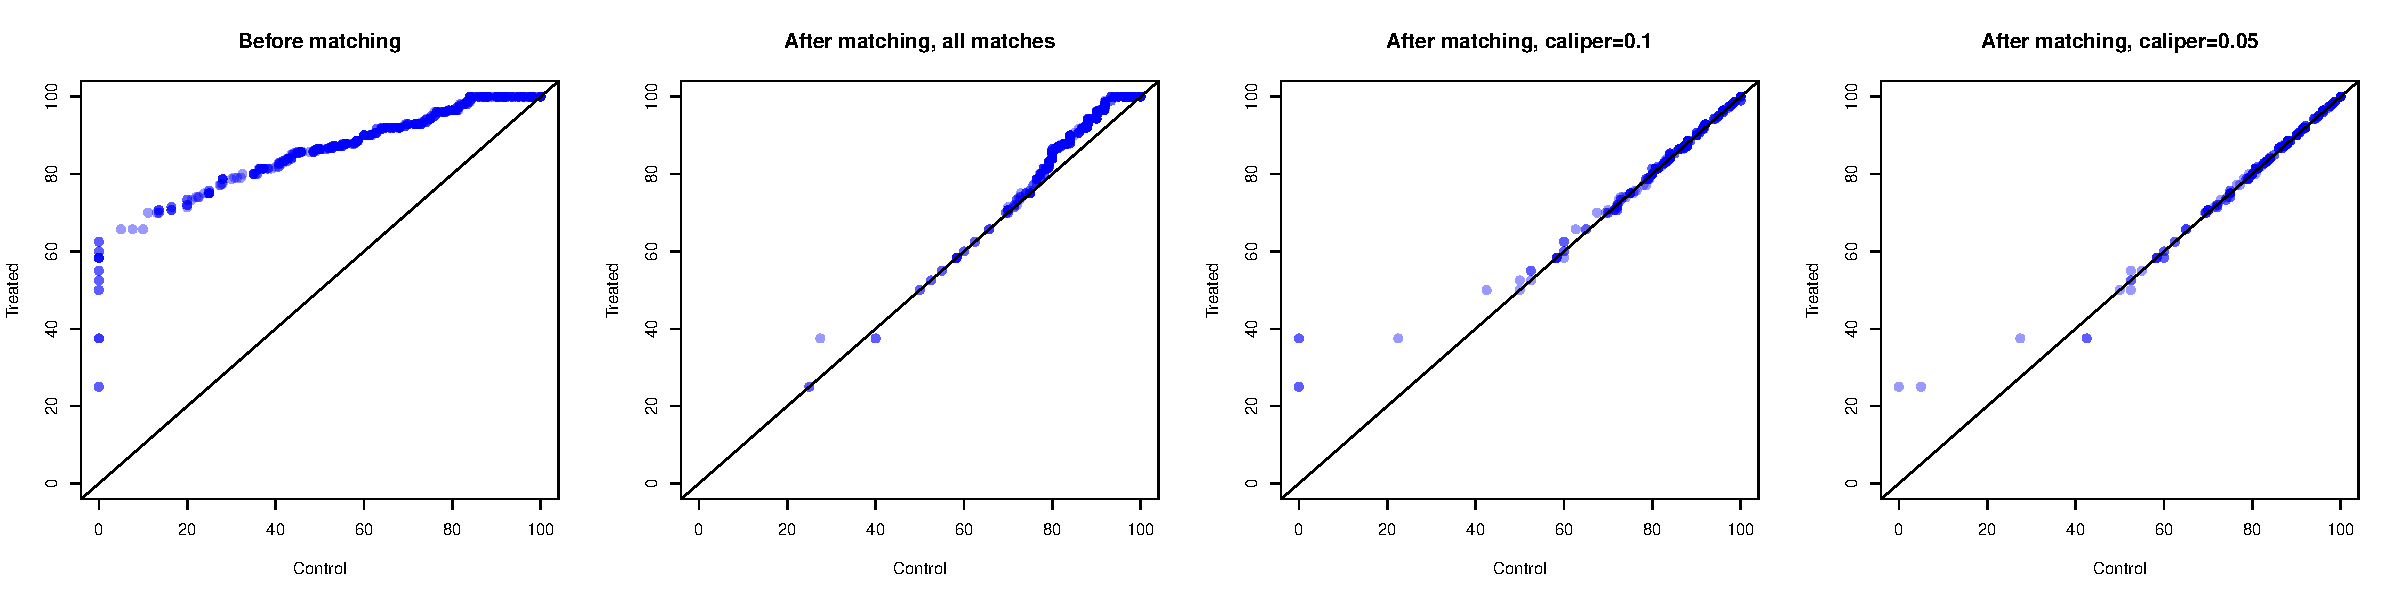
\includegraphics[width=.7\textwidth]{plots_type_3.pdf}
     \end{subfigure}
\end{center}
\end{minipage}
\end{figure}
\end{landscape}

\end{document}
